\documentclass[10pt,onecolumn,draftcls]{IEEEtran}
%\usepackage[bottom=20mm,left=20mm,right=20mm,top=20mm]{geometry}
\usepackage{pgfplots}
\usepackage{tikz}
\usepackage[utf8x]{inputenc}
\usepackage[L7x]{fontenc}
\usepackage[lithuanian]{babel}
\usepackage{epstopdf}
\usepackage{listings}
\usepackage{dsfont}
\usepackage{amsmath,amssymb}

\author{Maksim Norkin\\Vilniaus Gedimino technikos
  universitetas\\Elektronikos fakultetas\\Elektroninių sistemų katedra\\\texttt{maksim.norkin@ieee.org}}
\title{Bakalauro baigiamasis darbas\\Parkinsono ligos eigos stebėjimo priemonė}

\lstset{
  language=Matlab,
  basicstyle=\footnotesize,
  numbers=left
}

\begin{document}

\maketitle

\section{Įvadas. Užduoties analizė}

Darbo tema yra Parkinsono ligos eigos stebėjimo programa. Parkinsono
liga yra dažniausiai pasitaikantis neurodegeneracinis judėjimo
sutrikimas. Ankstyva ligos diagnozė ir efektyvus terapijos terapijos
stebėjimas yra būtinas pacientų gydymui ir sveikatos priežiūros kainai
sumažinti. Šiuo metu neegzistuoja gydytojų patvirtintos objektyvios ir
vieningos vertinimo sistemos, kuri tiksliai atpažintų Parkinsono ligos
simptomus. Vienas iš didžiausiai pasireiškiančių simptomų yra eisenos
sutrikimas. Sutrikimo dažnumą r svarbą patvirtina ir viešai prieinama
duomenų bazė, kurioje yra pateikiami sveikų ir sergančių Parinsono
liga žmonių eisenos duomenys. Duomenų bazė vadinasi "PhysioBank".

Darbo tikslas yra sukurti programą, gebančią atpažinti jėgos
jutikliais gautus signalus, priklausančius Parkinsono liga sergantiems
pacientams. Programa bus paremta Matlab platforma. Tokia platforma
buvo pasirinkta dėl didelių įrankių kiekių, kuris yra prieinamas
Matlab aplinkoje. Taip pat sekančioje platformoje yra labai patogu ir
greita realizuoti signalų apdorojimo sistemas d4l jos architektūros -
visi kintamieji yra matricos, kas yra labai patogu. Jėgos jutikliai
parodo vertikalią žemės reakcijos jėga (VŽRJ) (angl. Vertical Ground
Reaction Force (vGRF)). Fizikoje, ir būtent biomechanikoje, VŽRJ
nurodo kokia jėga žemė atsako ją slegiančiam objektui. Kaip
pavyzdžiui, stovinti žmogus slegia žemę jėga, kuri lygi jo masei ir
tuo pat metu, žemė slegia žmogų priešinga, lygiai tokia pačia
jėga. Parkinsono liga buvo pasirinkta dėl to, kad šiuo metu ji yra
aktyviai tiriama, kadangi visuomenė moka labai didelius pinigus
Parkinsono liga sergantiems asmenims. Per metus ši suma gali siekti 6
bilijonus dolerių. Ligos rizika su amžiumi tik didėja, todėl
analitikai prognozuoja, kad ateityje visuomenė mokės žymiai daugiau
dėl žmonių populiacijos senėjimo.

Didžiausia ligos atpažinimo problema slypi savybių, kurios geriausiai
atskirs sergantį Parkinsono liga nuo sveiko, nesergančio asmens. Darbo
metu bus apžvelgtos kelios galimo savybės, kurios gali atskirti tokius
pacientus. Blogiausias galimas variantas būtų nelinijinė funkcija
atskirti didelių dimensijų duomenys. Geriausias galimas variantas būtų
mažos dimensijos duomenys (iki 3 dimensijų) ir linijiškai atskiriami
duomenys (kadangi linijinę funkciją realizuoti yra
lengviausia). Turint didelių dimensijų duomenis, planuojamos sistemos
aparatiniai reikalavimai automatiškai padidėja, kadangi būtina
apdoroji labai daug duomenų. Tokią problemą galima išspręsti
panaudojus dimensijų mažinimo algoritmus, kurių dažniausiai taikomi:
Principinių komponenčių analizė (angl. Principal Component Analysis
(PCA)), linijinė diskriminanto analizė (anl. Linear Discriminant
Analysis (LDA)). Metodai bus aptarti vėlesnėse skyriuose. Jie taip pat
vadinami dimensijų praskyrimo algoritmai. Jie yra taikomi, kuomet
duomenis yra atskirti netiesiškai. Duomenims, atskirtu tiesiniu
dėsniu, galima taikyti paprastą klasifikavimo algoritmą. Jeigu
duomenis taip ir nepavyksta atskirti tiesiškai, tenka taikyti
kompleksinį klasifikatorių, ko pasekoje gali labai sumažėti
klasifikavimo rezultatas. Darbe bus panaudotas Matlab platformoje
įgyvendintas įrankis, kuris skirtas suprojektuoti naują dimensijų
plokštumą, kurį įgyvendino Boitech Franc savo magistriniam
darbe. Darbas buvo apgintas 2000 metais, Čekijos technikos
universitete, Prahoje. Tiesinio sklidimo dirbtinių neuronų
klasifikatorių bus panaudotas iš Matlab "Neural Network Toolbox"
įrankio. Likusi sistemos dalis bus aprašyta šiame darbe. Problema kyla
pirminiam signalų apdorojimo pasirinkime: visą gaunamą signalą pilnai
perduoti ar taikyti slankiojančio lango principą ar kitais, logiškai
apibrėžtais būdais, apdoroti pirminį signalą.

Sukurtas produktas gebės pateikti paciento eisenos Parkinsono ligos
eigos įvertinimą arba pateikti tikimybę kiek pacientas gali sirgti
Parkinsono liga, neatsižvelgiant į kitus ligos simptomus: drebulys
(rankų, kojų, žandikaulio, galvos), standumas (galūnių arba liemens
sustingimas), bradikinezija (judesių lėtumas), pozicijos nestabilumas
(arba sutrikęs balansas). Pati programa veiks nerealiu laiku. Tai
reiškia, kad pirmiausiai duomenys bus surenkami, o vėliau įkeliami į
programą tolimesniam apdorojimui.

Darbo tema, Parkinsono ligos eigos stebėjimo programa, reiškia, darbo
rezultate bus sukurtas algoritmas, kuriuo bus parengta kompiuterinė
programa. Pačiam kompiuteryje turi būti veikiantis Matlab programinis
paketas. Programa bus rašoma Matlab 7.12.0 (R2011) versija su "Neural
Network Toolbox" įrankiu. Eigos stebėjimas reiškia, kad visuomet
egzistuoja neapibrėžtas, galimas programos netikslumas. Visiškai
programa remtis, diagnozuojant Parkinsono ligą nėra galima, kadangi,
kaip jau buvo minėta ankščiau - eigos sutrikimas nėra vienintelis
ligos požymis. Turi būti atlikti ir kiti tyrimai, norint tiksliai
diagnozuoti ligą.

Darbo objekto sudėtis yra asmeniniam kompiuteriui skirta programa,
jėgos jutiklių signalų generavimo programa. Kokiam kompiuteriui
programa bus rašoma, paminėta ankščiau. Jėgos jutiklių generavimo
programa (modulis) bus atsakinga už signalų nuskaitymą iš duomenų
bazės ir jų pateikimą sistemos algoritmui. Taip pat signalų generavimo
programa (modulis“ bus naudojamas programos demonstracinei versijai
įgyvendinti.

Kaip buvo minėta, duomenys sistemai bus pateikiami iš "PhysioBank"
duomenų bazės. Duomenys duomenų bazėje buvo surinkti diskretizuojant
signalus $100~Hz$ diskretizavimo dažniu. Kiekvienu laiko momentu, yra
įrašoma nauja eilutė į duomenų tekstinę bylą. Eilutę sudaro 19
skilčių:

\begin{itemize}
\item Skiltis 1 nurodo laiką (sekundėmis);
\item Skiltys 2-9 nurodo kairės kojos 8 jutiklių VŽRJ, Niutonais;
\item Skiltys 10-17 nurodo dešinės kojos 8 jutiklių VŽRJ, Niutonais;
\item Skiltis 18 nurodo kairės kojos suminę VŽRJ, Niutonais;
\item Skiltis 19 nurodo dešinės kojos suminę VŽRJ, Niutonais;
\end{itemize}

Duomenų bazės bylų pavadinimai, pavyzdžiui: "GaCo01\_02.txt" ar
"JuPt03\_06.txt", sudaryti nurodant duomenų rinkimų sesijų pavadinimus:
"Ga" - "Galit Yogev et al" (dual tasking in PD; Eur J Neuro, 2005),
"Ju" - "Hausdoff et al" (RAS in PD; Eur J Neuro, 2007), "Si" - "Silvi
Frenkel-Toledo et al" (Treadmill walking in PD; Mov Disorders,
2005). Toliau, "Co" nurodo kontrolinį subjektą arba nesergantį
Parinsono liga subjektą, "Pt" nurodo Parkinsonu sergantį
subjektą. Pirmas numeris nurodo subjekto identifikacinį numerį, po
brūkšnio einantis antras numeris nurodo subjekto duomenų rinkimo seką.

Programos veikimas bus vertinamas taiklumu ir jautrumu. Parametrai yra
apskaičiuojami iš pasikliovimo matricos. Taiklumas apskaičiuojamas:

\begin{equation}
Taiklumas = \frac{T_P + T_N}{T_P + F_P + T_N + F_N},
\end{equation}

kur $T_P$ - teisingai identifikuotų klasių skaičius, $T_N$ - teisingai
atmestų klasių skaičius, $F_P$ - klaidingai identifikuotų klasių
skaičius ir $F_N$ - klaidingai atmestų klasių skaičius.

Tikslumas apskaičiuojamas:

\begin{equation}
Tikslumas = \frac{T_P}{T_P + F_P}
\end{equation}

Programos veikimas grafiškai demonstruojamas kreive, kuri nurodo
subjekto tikimybę sirgti Parkinsono liga.

\section{Informacinių Parkinsono ligos diagnostikos sistemų apžvalga}

Šiame skyriuje bus apžvelgtos analoginės informacinės sistemos arba
bandymai sukurti sistemą, kuri, remiantis įvairių jutiklių pagalba,
gebėtų atpažinti Parkinsono ligą.

Pirmas darbas, kuris bus analizuojamas, yra "Biometrinė ir mobili
eisenos analizavimo sistema ankstyvai Parkinsono ligos diagnozei ir % TODO: ref
terapijai". 

Antras darbas, ...

Trečias darbas, ...

Ketvirtas darbas, ...

\section{Signalų analizės programos kūrimas}

Šiame skyriuje apžvelgsime kylančias problemas, kuriant signalų
analizės programa ir galimus jų sprendimus. Kiekvienas sprendimas bus
išnagrinėtas, apžvelgta jo metodika, taikymo problemos bei rezultatai.

% TODO: papildyti

\subsection{Bendros programos struktūrinės schemos sudarymas}

\begin{figure}[!t]
  \centering
  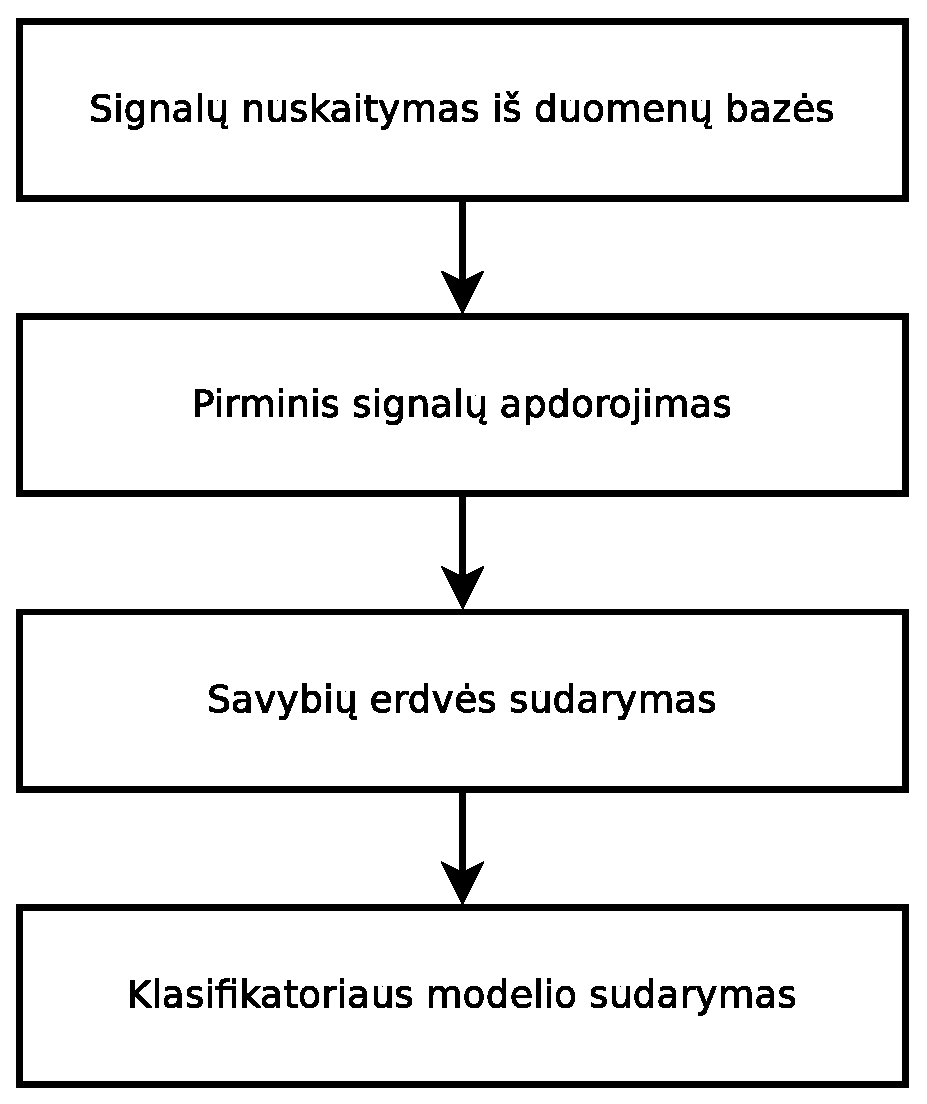
\includegraphics[width=200px]{figures/pirmine_schema.eps}
  \caption{Pirminė programos schema.}
  \label{fig:pirmine_programos_schema}
\end{figure}

Priklausomai nuo taikomos metodikos, programos struktūrinės schemos
skiriasi, kadangi vienas sprendimas reikalauja vieno tipo duomenų
struktūros, kitas - kitos struktūros. Programos projektavimo metu buvo
išbandyti keli programos variantai ir suprastinus veikimo schemas,
kiekvienas iš programos variantų veikė pagal bendrą schemą, kurią
galima apibrėžti \ref{fig:pirmine_programos_schema} pav. Reikalaujama,
kad kiekvienas iš algoritmų blokų būtų nepriklausomas nuo žemiau ar
aukščiau einančio bloko, kas reiškia, kad "Pirminio signalų
apdorojimo" bloko algoritmo pakeitimas neturi turėti jokios įtakos po
jo einančiam "Savybių erdvės sudarymas" blokui. 

Kiekvieno bloko užduotis:

\begin{enumerate}
\item "Duomenys iš duomenų bazės" bloko užduotis yra nuskaityti iš
  naudojamos "PhysioBank" duomenų bazės duomenis ir juos įkrauti į
  Matlab aplinką. Kadangi duomenys pateikiami tekstiniu pavidalu,
  Matlab aplinkoje yra labai patogi funkcija tokiems duomenims
  nuskaityti - $dlmread$.
\item "Pirminis signalų apdorojimas" bloko užduotis yra pradinis
  signalų filtravimas, nuolatinės komponentės pašalinimas. Taip pat, į
  šį bloką įeina ir atskirų signalų išskyrimas iš bendrai gaunamo
  signalo: signalo išskyrimas kuomet koja turi susilietimą su žeme,
  signalo išskyrimas, kuomet koja praranda susilietimą su žeme. Į
  bloką taip pat įeina ir slankiojančio lango algoritmo taikymas.
\item "Savybių erdvės sudarymas" bloko paskirtis yra pateikti
  pasirinktam klasifikatoriui išskirtas signalų savybes po pirminio
  signalo apdorojimo. Tokiomis savybės gali būti signalų dažninės
  komponentės (Furjė koeficientai), koreliacijos koeficientai tarp
  dešinės ir kairės kojos, savi-koreliacijos koeficientai dešinės ar
  kairės kojos. Detaliau nagrinėjamas savybes bus aptartos
  tolimesniuose poskyriuose. Į bloką taip pat įeina ir darbas su
  dimensijomis - dimensijų skaičiaus mažinimas ar naujos erdvės
  paieška, kurioje nagrinėjami duomenys yra geriau tiesiškai
  atskiriami.
\item "Klasifikatoriaus projektavimas" bloko paskirtis yra
  klasifikatoriaus apmokymas ir jo testavimas. Klasifikatoriaus
  pasirinkimas yra labai svarbus klausimas nagrinėjamam darbe. Jis
  turi būti parinktas argumentuotai, pateikiant detalius klasifikavimo
  rezultatus, remiantis rezultato grafiku. Nepasitikėjimo matrica, bei
  iš jos apskaičiuotais įverčiais: taiklumu bei tikslumu. Dar svarbus
  klasifikatoriaus aspektas yra savybių erdvės bendro dėsnio radimas
  arba jo aproksimacija. Šį faktą galima apibrėžti iš klasifikavimo
  grafiko. Jeigu klasifikavimo rezultatas yra nestabilus, ilgą laiką
  neturintis pastovaus rezultato, vadinasi, galima teigti, kad
  klasifikatorius blogai atliko erdvės dėsnio aproksimavimą, jis nėra
  tinkamas nagrinėjamai savybių erdvei.
\end{enumerate}

Tolimesniuose poskyriuose bus aptarti įgyvendinti blokinės struktūros elementai.

\subsection{Pirminio signalų apdorojimo programos kūrimas}

Šiame skyriuje bus aptartas pirminio signalų apdorojimo programos
kūrimas. Aptartas duomenų nuskaitymas iš duomenų bazės bylos
tekstiniame pavidale, galimas signalo išskaidymas slankiojančio lango
metodu arba signalo formos nuskaitymas, priklausomai nuo žinomo
fizinio poveikio, kuriuo metu signalas buvo gautas.

Programos kūrimo patogumui, buvo parinkta direktorijų architektūra:

\begin{itemize}
\item Tėvinė direktorija
  \begin{itemize}
  \item <programos versija, nurodyta datos formatu>
  \item database
  \item cache
  \end{itemize}
\end{itemize}

Kadangi programos kūrimo metu yra svarbu saugoti ankstesnes programos
versijas, buvo parinktas kasdienis programos versijos saugojimas:
kiekvienos pradžioje darbas buvo pradedamas su ankstesnės dienos
kopija. Taip buvo išsaugotas kiekvienos darbo dienos programos versija
ir taip galima peržiūrėti kokiu analitiniu keliu buvo eita prie
dabartinės programos versijos.

Pirmoji funkcija, priklausanti pirminio signalo apdorojimo programai
yra $read\_data$. Funkcijos kodas pateikiamas \ref{code:read_data} pav.

\begin{figure}[t]
  \centering
  \lstinputlisting{sources/read_data.m}
  \caption{Duomenų nuskaitymo funkcija iš tekstinės duomenų bylos.}
  \label{code:read_data}
\end{figure}

Funkcijai užtenka nurodyti tik norimos nuskaityti bylos pavadinimą,
kaip pavyzdžiui "SiPt30\_01.txt" ir funkcija gražins kairės kojos
duomenis. Duomenų analizėje naudojami tik vienos kojos duomenis,
kadangi dešinės ir kairės kojos duomenys yra stipriai koreliuoti, % TODO: ref
todėl nėra prasmės naudoti dviejų kojų duomenų. Pasirinkus tokį
sprendimą taip pat yra sumažinamas skaičiavimų skaičius
programoje. Duomenų bazės direktorija nurodyti kintamojo vietoje yra
taip pat svarbus aspektas, kadangi pakitus duomenų bazės vietai,
užteks tik pakeisti vieną kintamąjį, o ne visą kodą, nors kodas ir
nėra ilgas. Matlab funkcija $dlmread$ gražina duomenis masyvo
pavidalu, kur stulpelis nurodo įvade aptartus duomenis, o eilutė
nurodo duomenų vertes tam tikru laiko momentu.

\begin{figure}[t]
  \centering
  \lstinputlisting{sources/split_data.m}
  \caption{Slankiojančio lango algoritmo pritaikymas.}
  \label{code:sliding_window}
\end{figure}

Sekantis žingsni, po duomenų nuskaitymo, yra jų pirminis
apdorojimas. Nagrinėjimas bus pradėtas nuo slankiojančio lango
metodo. Programos kodas pateikiamas \ref{code:sliding_window}
pav. Funkcijos įvestyje pateikiamas nagrinėjamas signalas, slankiojamo
lango ilgis ir slankiojamo lango perdanga. Slankiojamo lango perdanga
nurodo reikšmių arba laiko verčių kiekį, kurį algoritmas pašalina iš
spartinančiosios atminties, laukdamas naujų verčių langui
užpildyti. Pavyzdžiui, jeigu lango ilgis yra 4 signalo verčių, o
perdanga - 2 signalo vertės, vadinasi, kai algoritmas užpildys langą 4
signalo vertėm, esamą langą jis perduos į išėjimo spartinančiąją
atmintį, paskutines dvi vertes ištrins iš spartinančiosios atminties
ir iš naujo lauks naujų dviejų reikšmių langui pilnai užpildyti.

Funkcija yra tiek lanksti, kad nėra svarbu kokio tipo duomenys yra
pateikiami - ar tai konkretaus signalo vertės ar iš ankščiau
pritaikyto slankiojančio lango algoritmo išskirtos signalo savybės,
kuriuos buvo panaudotos formuojant naują signalą. Tokia funkcijos
savybė bus labai naudinga tolimesniame darbe.

\begin{figure}[t]
  \centering
  \begin{lstlisting}
    [B,A] = butter(9, 1/50, 'high');
    [BB,AA] = butter(9, 40/50, 'low');
    output = filter(BB, AA, filter(B, A, input));
  \end{lstlisting}
  \caption{Signalo filtravimas dviem Butterworth filtrais.}
  \label{code:filter}
\end{figure}

Sekanti programos dalis atlieka paprastą signalo filtravimą su dvejais
$Butterworth$ skaitmeniniais filtrais. Pirmasis, aukštų dažnių
filtras, skirtas pašalinti signalo nuolatinei komponentei. Antras,
žemų dažnių filtras, skirtas pašalinti aukšto dažnio triukšmą, kuris
neneša visiškai jokios naudingos informacijos. Filtras įgyvendinamas
labai paprastai. Kodo pavyzdys pateikiamas \ref{code:filter}
pav. Abiejų filtrų eilė yra 9-ta, žemų dažnių filtro ribinis dažnis
parinktas $40~Hz$. Duomenys diskretizuojami $100~Hz$ dažniu, vadinasi
didžiausias galimas signalo dažnis yra $50~Hz$. Didžiausias žmogaus
generuojamas dažnis ėjimo metu, remiantis šaltiniu, yra $20~Hz$. % TODO: ref
Užtikrintumui buvo parinktas $40~Hz$ dažnis. Nuolatinė dedamoji
pašalinama su aukšto dažnio filtru, kurio ribinis dažnis yra
$1~Hz$. Nuolatinė dedamoji neneša jokios informacijos apie eisena,
kadangi ji tiktais nurodo naudojamų jutiklių jautrumą.

\begin{figure}[t]
  \centering
  \lstinputlisting{sources/extract_signal.m}
  \caption{Kontakto su žeme signalo išskyrimo programos kodo fragmentas.}
  \label{code:signal_extraction}
\end{figure}

Toliau seka, priklausomai nuo pasirinkto pirminio signalų apdorojimo
būdo, signalo išskyrimas pagal fizinę veiklą. Dominančios signalo
būsenos yra, kai subjekto koja turi kontaktą su žeme ir nurodytas
subjektas neturi kontakto su žeme. Kontakto su žeme signalo išskyrimui
programos kodas yra pateikiamas \ref{code:signal_extraction} pav.

Pirmiausiai, "Pt\_t" kintamojo struktūroje yra saugoma kairės kojos
Parkinsono liga sergančių subjektų duomenys. Kiekvienas signalas yra
priskiriamas prie $signal$ kintamojo, su kuriuo toliau yra tęsiamas
apdorojimo procesas. Jeigu signalas nėra lygus nuliui, tuomet jis
įdedamas į laikinąją atmintį. Taip signalas yra tikrinamas iki tol,
kol signalas tampa lygus nuliui ir tęsiamas tolimesnis
apdorojimas. Apdorojimas susideda iš signalo ilgio patikros. Jeigu
signalas yra trumpesnis už 10 verčių, arba turint omenyje, kad
signalas buvo diskretizuojamas $100~Hz$, tai $0.1~s$, vadinasi,
signalas yra tiesiog aukšto dažnio triukšmas arba blogas pavyzdys ir
signalas yra atmetamas. Jeigu signalas yra ilgesnis už 200 verčių
($2~s$), vadinasi, duomenų rinkimo metu įvyko klaida ir koja per tokį
laiką pakelta nebuvo. Tokia klaida gali būti sukelta, kuomet subjektas
ne eina, o stovi ant dviejų kojų arba tik ant kairės kojos. Jeigu visi
kriterijai patenkinami, signalas yra priimamas ir kraunamas į
laikinąją atmintį, pavadinimu "$data.Pt$". Signalas, kuriuo metu koja
neliečia žemės, yra randamas kartu su ankščiau išnagrinėtu
metu. Algoritmas patikrina kiek praėjo laiko (arba kiek verčių yra
priskaičiuota) nuo paskutinio užskaityto kojos ant žemės signalo ir
įrašo tą signalą į laikiną atmintį, jeigu po praeito signalo nepraėjo
mažiau negu 50 verčių arba $0.5~s$ ir nedaugiau nei 200 verčių arba
$2~s$. Kojos signalas yra pateiktas \ref{fig:stance_phase} pav.

\begin{figure}[t]
  \centering
  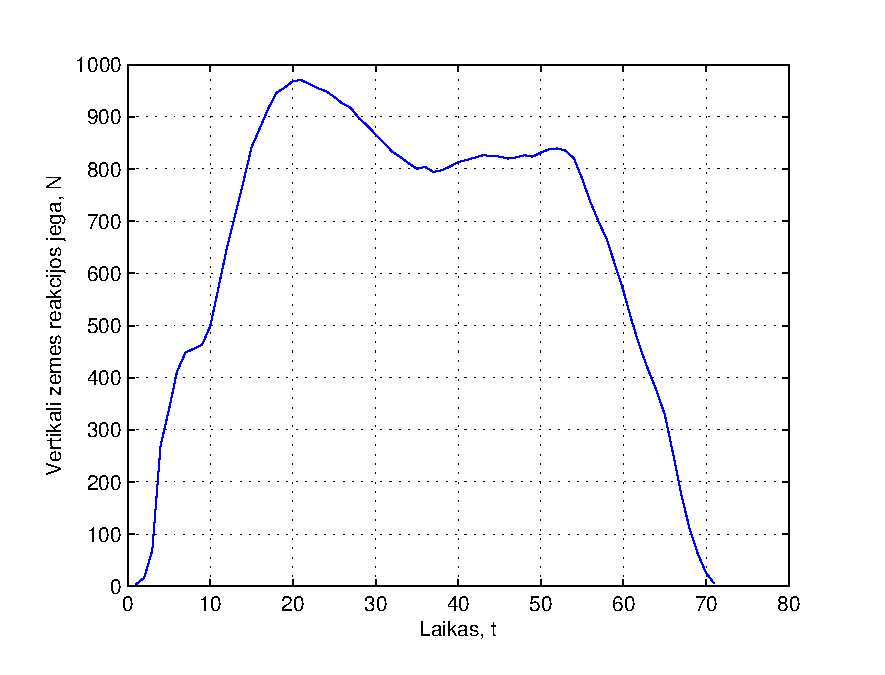
\includegraphics[width=300px]{figures/09_sample_stance_phase.eps}
  \caption{Susilietimo su žeme signalas.}
  \label{fig:stance_phase}
\end{figure}

\begin{figure}[t]
  \centering
  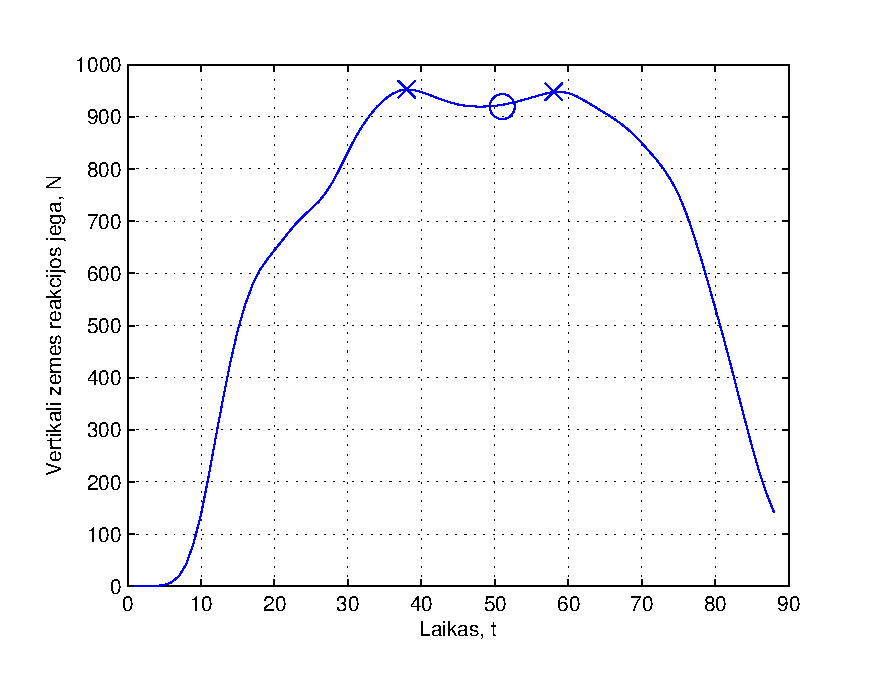
\includegraphics[width=300px]{figures/10_global_max_local_min.eps}
  \caption{Dviejų globalių maksimumų ir vieno lokalaus minimumo
    radimas signale.}
  \label{fig:min_max}
\end{figure}

Dar vienas pirminis signalo apdorojimas, kurį teko panaudoti tiriant
galima bendrą erdvę - kiekvieno kojos susilietimo su žeme signalo
dviejų globalių maksimumų ir vieno lokalaus minimumo
paieška. Algoritmo rezultatas yra pateiktas \ref{fig:min_max}
pav. Kryžiais pažymėtos globalaus maksimumo vietos, apskritimu
pažymėta lokalaus minimumo signalo vieta. Išanalizavus daugumos
subjektų žingsnio signalus, buvo padaryta išvada, kad kiekviename
žmogaus žingsnyje egzistuoja du maksimumai. Vienas maksimumas
randamas, kai subjektas yra visiškai atsirėmęs galine pėdos dalimi į
žemę, antras maksimumas randamas, kai subjektas visiškai atsiremia
priekinę pėdos dalimi. Tarp šių dviejų maksimumų yra pereinamasis
laikotarpis, kuris yra signalo lokalus minimumas. Priežastis, dėl
kurios algoritmas buvo įgyvendintas, yra vienas darbas, kuriame % TODO: ref
buvo pasiūlyta naudotis būtent tokiomis savybėmis atpažinti Parkinsono
liga sergančius subjektus nuo nesergančių subjektų. Pačio algoritmo
kodo dalis yra pateikta \ref{code:min_max} pav.

\begin{figure}[t]
  \centering
  \lstinputlisting{sources/min_max.m}
  \caption{Dviejų globalių maksimumų ir vieno lokalaus minimumo radimo
  algoritmo fragmentas.}
  \label{code:min_max}
\end{figure}

Programos kodas krauna gaunamą signalą į laikinąją atmintį ir tikrina
ar signalas pakito per užduotą dydį $\delta$. Delta nurodo kiek
signalas turi pakisti, kad algoritmas nuspręstų, kad signalas pradėjo
mažėti. Tokio tikrinimo priežastis yra ta, kad prieš globalų maksimumą
taip pat yra sritis, kurioje signalas kilimas sulėtėja, o kai kuriuose
pavyzdžiuose buvo pastebėta, kad signalas net pradeda mažėti. Dėl šios
priežasties buvo įvesta pokyčio tikrinimo sąlygą.

Pirminio signalų apdorojimo programa baigiasi nurodytais
metodais. Sekantis žingsnis yra apdorotų duomenų perdavimas tolimesnei
programos pakopai - požymių išskyrimui.

\subsection{Požymių išskyrimo programos kūrimas}

Požymių išskyrimas priklauso nuo pirminio signalo apdorojimo
mechanizmo. Jeigu ankstesniame bloke pakeisime ribinį filtro dažnį ir
kaip nagrinėjamą požymį bus parinktas koreliacijos koeficientai ar
dažninės komponentės - požymio vektorius pakis, todėl prieš kiekvieną
požymių analizavimo ciklą bus pateikta ir pirminiam signalų apdorojimo
bloke naudojami metodai. Taip pat, kadangi požymių išskyrimo programos
kūrimas taip pat sprendžia ir dimensijų klausimą - skyriaus pradžioje
bus trumpai apžvelgti populiariausi šiame darbe panaudoti dimensijų
mažinimo metodai.

\subsubsection{Dimensijų mažinimas}

Dimensijų mažinimas suteikia dideles galimybes supaprastinti
klasifikavimo uždavinį. Kuomet duomenys savybių erdvėje nėra
linijiškai atskirti, yra sunku nustatyti ar klasifikatorius ras
apibendrintą duomenų praskyrimo funkciją. Norint užtikrinti, kad
klasifikatorius veiks teisingai - yra atliekamas dimensijų
praskyrimas. Metodas taip pat taikomas, kuomet norima sumažinti
dimensijų skaičių. Problema iškyla, kuomet norima įgyvendinti sukurtą
sprendimą įterptinėje sistemoje, kurioje negalima pasiekti didelių
aparatinių resursų. Turint didelių dimensijų duomenis taip pat kyla ir
pačios sistemos kaina, dėl tų pačių aparatinių resursų
reikalavimų. Norint išvengti tokių problemų - taikomi dimensijų
mažinimo algoritmai. Populiariausi dimensijų mažinimo algoritmai yra:

\begin{itemize}
\item Linijinė diskrtiminanto analizė (angl. Linear Discriminant
  Analysis (LDA));
\item Principinė komponenčių analizė (angl. Principal Component
  Analysis (PCA)).
\end{itemize}

Taip pat, kiekvienas iš paminėtų būdu taip pat gali būti papildytas
branduolio (angl. Kernel) funkcija. Metodų apibūdinimas bus pradėtas
nuo paprasčiausios iš dviejų - PCA.

Principinė komponenčių analizė yra statmena ir paprasta
transformacija, kuri yra daug kur naudojama dėl paprastos matematinės
pusės ir lengvo įgyvendinimo. Egzistuoja skirtingi PCA metodo
įgyvendinimo algoritmai. Vienas iš jų yra vienetinės reikšmės
skaidymas (angl. Singular Value Decomposition (SVD)). Literatūroje PCA
ir SVD dažniausiai minimi kaip sinonimai. SVD yra greitas, tačiau
didelių atminties resursų reikalaujantis metodas. Kuomet dideli
atminties resursai nėra prieinami (įterptinėje sistemoje), reikia
naudoti kitą įgyvendinimo variantą - naudoti tikrinių vektorių
skaidymą. Toks sprendimas užima didesnius laiko resursus, lyginant su
SVD, tačiau jam reikia mažesnių atminties resursų ir jis tinka
nagrinėti didelių dimensijų duomenis. Toks sprendimas bus taikomas ir
šiame darbe. PCA įgyvendinimas naudojant SVD ir tikrinių vektorių
skaidymą yra pateiktas priede. Toliau bus išnagrinėtas PCA iš % TODO: appendix
matematinės pusės.

Matematiškai, PCA apibrėžiamas kaip statmena linijinė transformacija,
kuri transformuoja duomenis į naują koordinačių sistemą, kurioje
didžiausią variaciją projektuojama į pirmą ašį, antroji didžiausia
variacija (statmena pirmajai) projektuojama į antrą ašį. Procesas
tęsiasi tol, kol yra pasiekiamas norimas dimensijų skaičius.

Apibrėžta duomenų matrica $\textbf{X}^T$, su empiriniu vidurkiu, kuris
lygus nuliui (empirinis vidurkis reiškia vidurkio apskaičiavimą ir jo
atėmimą iš duomenų), kur kiekviena eilutė $n$ atspindi duomenų
rinkinį, o stulpelis $m$ - turimas duomenų dimensijas. Matricos
$\textbf{X}$ vienetinės reikšmės skaidymas išreiškiamas:

\begin{equation}
  \mathbf{X} = \mathbf{W} \Sigma \mathbf{V}^T,
\end{equation}
kur $m*n$ matrica $\mathbf{W}$ yra matricos $\textbf{XX}^T$ tikrinių
vektorių matrica, $\Sigma$ matrica yra $m*n$ stačiakampio įstrižainės
matrica su realiais skaičiais įstrižainėje ir $n*n$ tikrinių vektorių
$\mathbf{X}^T\mathbf{X}$ matrica $\mathbf{V}$. PCA transformacija,
kuri sukonstruoja naujas dimensijas, yra apibrėžiama:

\begin{equation}
  \mathbf{Y}^T = \mathbf{X}^T \mathbf{W} = \mathbf{V} \Sigma^T
  \mathbf{W}^T \mathbf{W} = \mathbf{V} \Sigma^T .
\end{equation}

Kadangi $\textbf{W}$ yra statmena matrica, kiekviena $\textbf{Y}^T$
eilutė yra matricos $\textbf{X}^T$ eilutės sukimas. Pirmasis
$\textbf{Y}^T$ stulpelis yra pirmosios komponentės rezultatas, antras
stulpelis yra antrosios komponentės rezultatas. Kiek stulpelių
$\textbf{Y}^T$ turi, tiek ir rezultatų (dimensijų) yra po
transformacijos.

Linijinė diskriminanto analizė yra dimensijų mažinimo metodas (kuris
kartu yra naudojamas kaip ir klasifikatorius), yra vienas iš metodų,
kuris neša kartu ir duomenų žymėjimo informaciją. Tai reiškia, kad
mažinant dimensijų skaičių, metodas turi žinoti kokie duomenys
priklauso kokiai duomenų klasei. Pagrindinis LDA tikslas yra didinti
sekantį kriterijų:

\begin{equation}
  \mathfrak{J}(\mathbf{w}) = \frac{ \mathbf{w}^T S_B \mathbf{w} }{
    \mathbf{w}^T S_W \mathbf{w} },
\end{equation}
kur $S_B$ yra "išorinės klasės scatter matrica", $S_W$ yra "vidinė
klasės scatter matrica". Scatter matricų apibrėžimas yra:

\begin{equation}
  S_B = \sum_c (\mu_c - \bar{x})(\mu_c - \bar{x})^T
\end{equation}

\begin{equation}
  S_W = \sum_c \sum_{i \in c} ( x_i - \mu_c)(x_i - \mu_c)^T
\end{equation}

\subsubsection{Savybių tyrimas}

Šiame skyriuje bus išnagrinėtos galimos signalų savybės, pagal kurias
galima atskirti Parkinsono liga sergantį subjektą nuo sveiko
subjekto. Kaip buvo minėta ankščiau, ne visos savybės gali būti
išskirtos, naudojantis vienu pirminio signalo apdorojimo mechanizmu,
todėl kiekvienos savybės nagrinėjimo pradžioje bus paminėta ir
pirminio signalo apdorojimo bloko sudėtis.

Galimų savybių analizavimas gali būti pradėtas nuo signalo dažninių
komponenčių (Furjė transformacijos). Kaip nurodo šaltiniai, % TODO: reference
Parkinsono liga sergančių subjektų žingsniai turi statesnius šlaitus,
kas iš signalų apdorojimo srities reiškia, kad signalas turi turėti
aukštas dažnines komponentes. Šiai savybei išskirti pirminiam signalo
apdorojimo bloke bus panaudotas slankiojančio lango metodas. Taip
kiekvienas signalas turės fiksuotą ilgį ir taip bus galima lyginti
signalus tarpusavyje.

\begin{figure}[t]
  \centering
  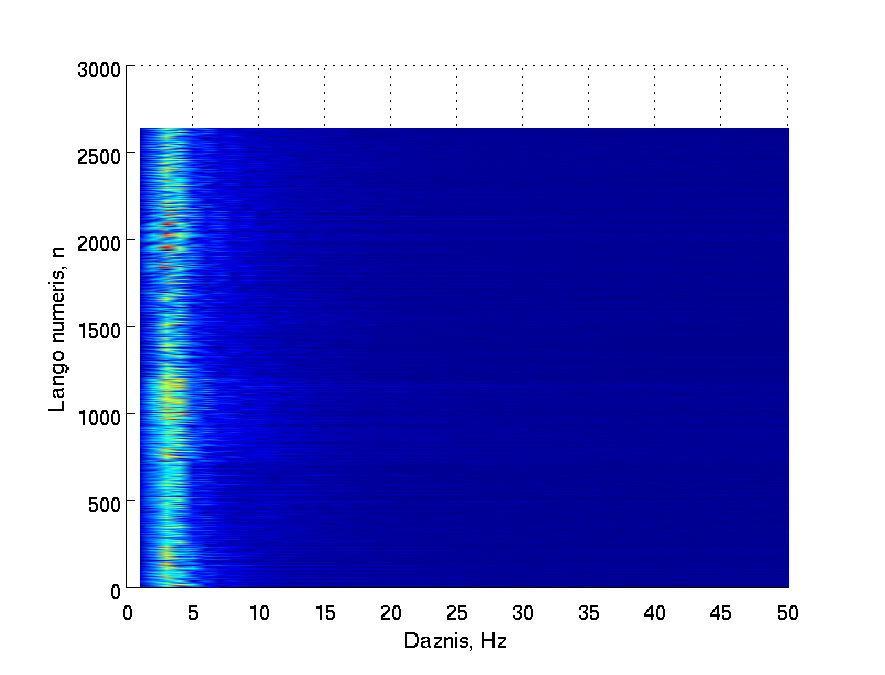
\includegraphics[width=300px]{figures/co_fft.eps}
  \caption{Kontrolinių subjektų kairės kojos žingsnių signalų dažninės
  komponentės}
  \label{fig:co_fft}
\end{figure}

\begin{figure}[t]
  \centering
  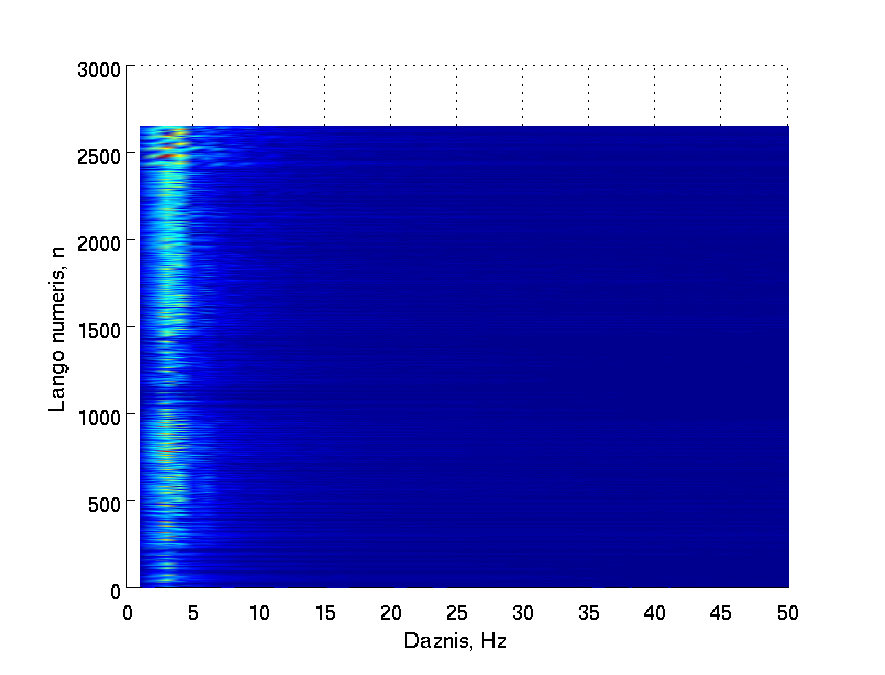
\includegraphics[width=300px]{figures/pt_fft.eps}
  \caption{Parkinsono liga sergančių subjektų kairės kojos žingsnių signalų dažninės
  komponentės}
  \label{fig:pt_fft}
\end{figure}


Toliau bus išanalizuoti Parkinsono liga sergančių subjektų ir
kontrolinių subjektų žingsnių signalų dažninės
komponentės. Kontrolinių subjektų kairės kojos žingsnių dažninės
komponentės yra pateiktos \ref{fig:co_fft} pav. Parkinsono liga
sergančių subjektų kairės kojos žingsnių dažninės komponentės yra
pateiktos \ref{fig:pt_fft} pav. Kaip matoma iš duotų komponenčių
grafikų - tiek kontrolinių subjektų, tiek Parkinsono liga sergančių
subjektų pagrindinės dažninės komponentės išsidėsto iki $5~Hz$
ruože. Ties $0~Hz$ dažninių komponenčių nėra, kadangi jos buvo
pašalintos filtro pagalba. Už $10~Hz$ ribos, komponentės neneša
visiškai jokios informacijos. Iš to galima padaryti išvadą, kad tiek
Parkinsono liga sergančių subjektų, tiek kontrolinių subjektų eisenos
yra visiškai vienodos dažnių srityje ir vien remiantis šita
informacija nėra galima nustatyti ar subjektas serga Parkinsono liga
ar ne.

Tolimesnė analizė gali būti atlikta, remiantis koreliacijos
koeficientais. Analizuojant šias savybes, galima remtis tokiu pačiu
pirminiu signalo apdorojimo bloku, kaip ir analizuojant dažnines
komponentes. Dėl to, kad esama tikrais kairės kojos sinalai, alima
taikyti tik savi-koreliacijos koeficientus. Narinėjama savybė parodė
labai gerus rezultatus ankstesniame tyrime, kuriame, remiantis
akselerometro ir giroskopo jutiklių parodymais, reikėjo suprojektuoti
algoritmą, gebantį atskirti tokias žmogaus veiklas: stovėjimas,
ėjimas, ėjimas aukštyn laiptais, ėjimas žemyn laiptais.

\begin{figure}[t]
  \centering
  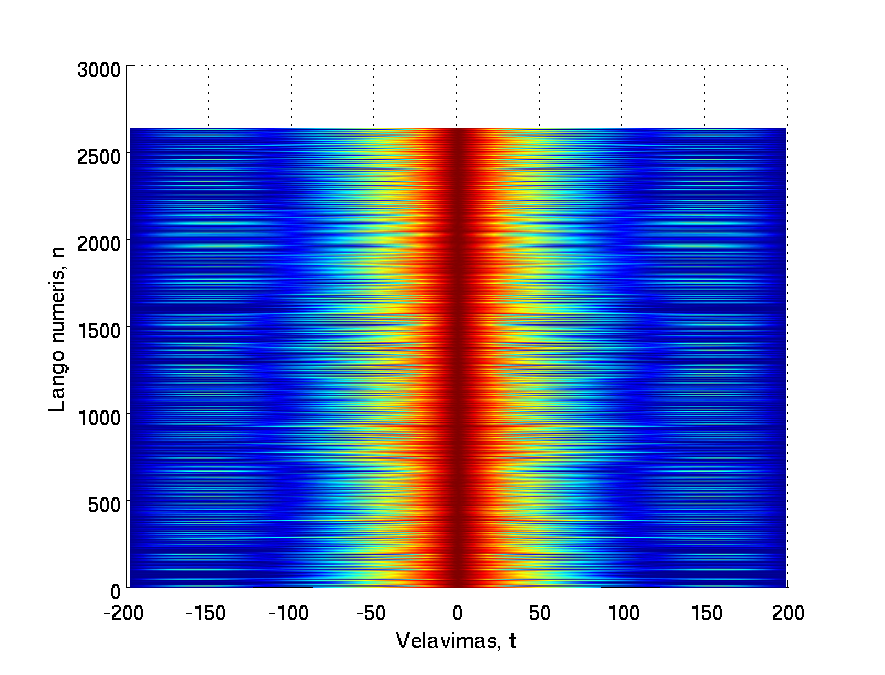
\includegraphics[width=300px]{figures/co_corr.eps}
  \caption{Kontrolinių subjektų kairės kojos žingsnių signalų
    savi-koreliacijos koeficientai.}
  \label{fig:co_corr}
\end{figure}

\begin{figure}[t]
  \centering
  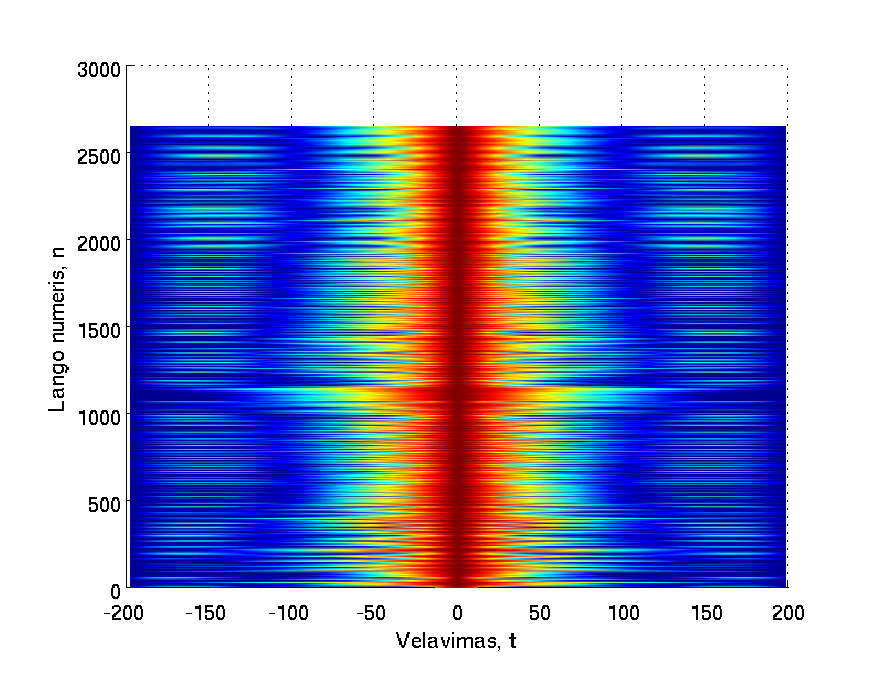
\includegraphics[width=300px]{figures/pt_corr.eps}
  \caption{Parkinsono liga sergančių subjektų kairės kojos žingsnių
    signalų savi-koreliacijos koeficientai.}
  \label{fig:pt_corr}
\end{figure}

Kontrolinių subjektų kairės kojos savi-koreliacijos koeficientai
parodyti \ref{fig:co_corr} pav. Parkinsono liga sergančių subjektų
kairės kojos savi-koreliacijos koeficientai parodyti \ref{fig:pt_corr}
pav. Kaip matosi iš korelogramos, tiek sergantys, tiek kontroliniai
subjektai turi panašias, o kai kuriais atvejais ir tokias pačias,
koreliacijos reikšmes. Remiantis vien tik turima informacija,
nustatyti ar subjektas serga Parkinsono liga ar ne, nėra įmanoma.

\begin{figure}[t]
  \centering
  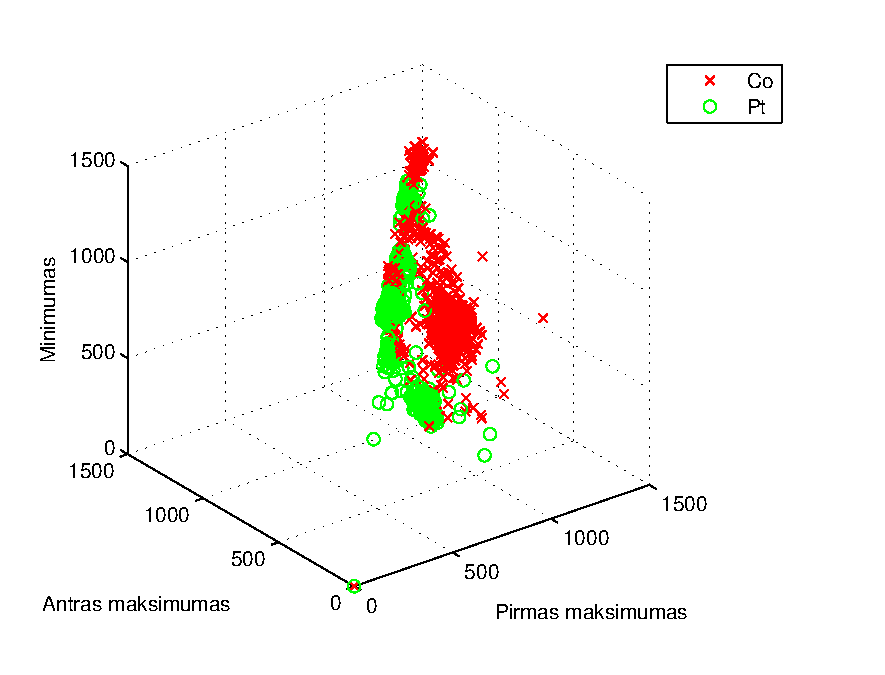
\includegraphics[width=300px]{figures/maximums_minimums.eps}
  \caption{Dviejų globalių maksimumų ir vieno lokalaus minimumo
    savybių erdvė.}
  \label{fig:max_min}
\end{figure}

Sudėtingesnė analizė seka iš dviejų globalių maksimumų ir vieno
lokalaus minimumo savybių erdvės. Šios tris savybės sudaro trijų
dimensijų plokštumą, kurią galima lengvai pavaizduoti. Pilna savybių
erdvė pavaizduota \ref{fig:max_min} pav. .

\subsection{Požymių klasifikavimo programos kūrimas}

\subsection{Duomenų analizės programos kūrimas}

\section{Signalų analizės programos įgyvendinimas}

Šiame skyriuje apžvelgsime įgyvendinta programinį kodą ir jo veikimo
architektūrą. Ankstesniuose poskyriuose buvo argumentuotai pažvelgti
galimi analizės metodai, požymiai ir klasifikatoriai. Visi rezultatai
bus panaudoti projektuojant galutinį sprendimą.

Poskyryje \ref{subsec:total_scheme} bus pateikta bendra programos
algoritmo veikimo schema, poskyryje \ref{subsec:class_scheme} bus
pateikta algoritmo klasifikavimo veikimo schema, poskyryje
\ref{subsec:total_program} bus apžvelgta galutinė programa.


\subsection{Bendro programos algoritmo schemos sudarymas}
\label{subsec:total_scheme}

Ankstesniame skyriuje buvo apžvelgta bendra programos veikimo
schema. Bendros schemos pavyzdys yra pateiktas
\ref{fig:pirmine_programos_schema} pav. Šiame  poskyryje bus patekta
detali algoritmo schema ir aptarta kiekviena jo bloko paskirtis, bei
jame naudojamas metodas.

\subsection{Požymių klasifikavimo programos algoritmo schemos
  sudarymas}
\label{subsec:class_scheme}

\subsection{Signalų analizės programos įgyvendinimas}
\label{subsec:total_program}

Šiame poskyryje 

\section{Signalų analizės programos patikra}

Šiame skyriuje bus parengtas ir įgyvendintas algoritmo patikros
planas. Patikra bus atliekama su užduoties analizėje nurodytais
duomenimis - ... Parkinsono liga sergančių asmenų ir ... nesergančių
asmenų duomenimis.

\subsection{Eksperimentų plano rengimas}

Detaliai ištiriant programos veikimo rezultatus, reikia nurodyti
programos įvestyje kiek galima daugiau galimų signalo analizės
scenarijų.

Galimi signalų apdorojimo scenarijai:

\begin{itemize}
\item Reikia pagalvoti;
\item Reikia pagalvoti.
\end{itemize}

\subsection{Duomenų eksperimentams rengimas}

\subsection{Programos patikros rezultatai}

Algoritmo patikros metu buvo gauti tokie rezultatai...

\bibliographystyle{plain}
\bibliography{references}

\end{document}
